\documentclass{article}
\usepackage[czech]{babel}
\usepackage[utf8]{inputenc}
\usepackage{graphicx}
\usepackage{pdfpages}
\usepackage{textgreek}
\usepackage{xargs} 
\usepackage{xcolor}
\usepackage{pdfpages}
\usepackage{cite}
\usepackage[colorinlistoftodos,prependcaption,textsize=tiny]{todonotes}
\newcommandx{\xtodo}[2][1=]{\todo[linecolor=red,backgroundcolor=red!25,bordercolor=red,#1]{#2}}


\usepackage{listings}
\usepackage{color}

\definecolor{dkgreen}{rgb}{0,0.6,0}
\definecolor{gray}{rgb}{0.5,0.5,0.5}
\definecolor{mauve}{rgb}{0.58,0,0.82}

\lstset{frame=tb,
  language=Sql,
  aboveskip=3mm,
  belowskip=3mm,
  showstringspaces=false,
  columns=flexible,
  basicstyle={\small\ttfamily},
  numbers=none,
  numberstyle=\tiny\color{gray},
  keywordstyle=\color{blue},
  commentstyle=\color{dkgreen},
  stringstyle=\color{mauve},
  breaklines=true,
  breakatwhitespace=true,
  tabsize=3
}




\begin{document}


%---------------------------------------------------------------------------------------------------------------------------------------------------------------%


\begin{titlepage}	
	\begin{center}
		
\includegraphics[width=5cm]{logo.jpg}\\[3.5cm]
		{\Huge KIV/VSS}\\[0.5cm]
		{\Large Semestrální práce}\\[0.5cm]
		{\large  Miroslav Liška – A17N0081P}\\[0.5cm]
		{\large  topiker@students.zcu.cz}\\[0.5cm]
		{\large   9.12.1992}\\[0.5cm]
		\vfill

		{\large \today}

	\end{center}
\end{titlepage}



\section{Zadání} %%%%%%%%%%%%%%%%%%%%%%%%%%%%%%%%%%%%%%%%%%%%%%%%%%%%%%%%%%%%%%%%%%%%%%%%%%%%%%%%%%%%%%%%%%%%%%%%%%%%%%%%%%%%%%%%%%%%%%%%%%%%%%%%%%%%%%%%%%
\setcounter{page}{1}
Cílem semestrální práce je vytvoření analytického výkonnostního nebo spolehlivostního modelu zadaného systému a jeho řešení.
 Dále vytvoření simulačního modelu pro tentýž problém a závěřem obě řešení porovnat.


\section{Analýza}

\subsection{Popis problému}
V rámci práce byl zvolen model inspirovaný jídelnou (menzou) na Borech. Navržený model je možné vidět na obrázku.\ref{fig:schema_menza}.

Schéma obsahuje jedno místo generování požadavků (S1).
 V reálném světě je míst generujících požadavků několik, nicméně se všichni musí dostat do budovi jednimi dveřmi.
Z tohoto důvodu je vstupní proud požadavků spojen do jednoho a tedy i jejich střední doby generování.
Strávnici se po vstupu hromadí na jednom místě - u turniketů.
Následně si jdou vyzvednout jídlo k jednomu z pultů. 
Každý pult má jednu frontu a každé jídlo se vydává na jednom místě.
Poté následuje placení, kde si student vybere jednu ze dvou pokladen. 
Po zaplacení by typicky následovalo stravování. 
Tato operace ale nebyla do simulace zahrnuta.
Student tedy po dokončení stravování může dostat ještě hlad a vrátit se tak na začátek k turniketům, nebo se vydá odevzdat tác.
Stroj s tácem zajištuje také právě jednu frontu.
V tuto chvíli strávník odchází ze zařízení, nebo má ještě hlad a vrací se zpět na začátek k turniketům.
Všechny kanály obsluhy jsou tedy typu M/M/1 a všechny fronty jsou typu FIFO.

	\begin{figure} [ht!]
		\centering
		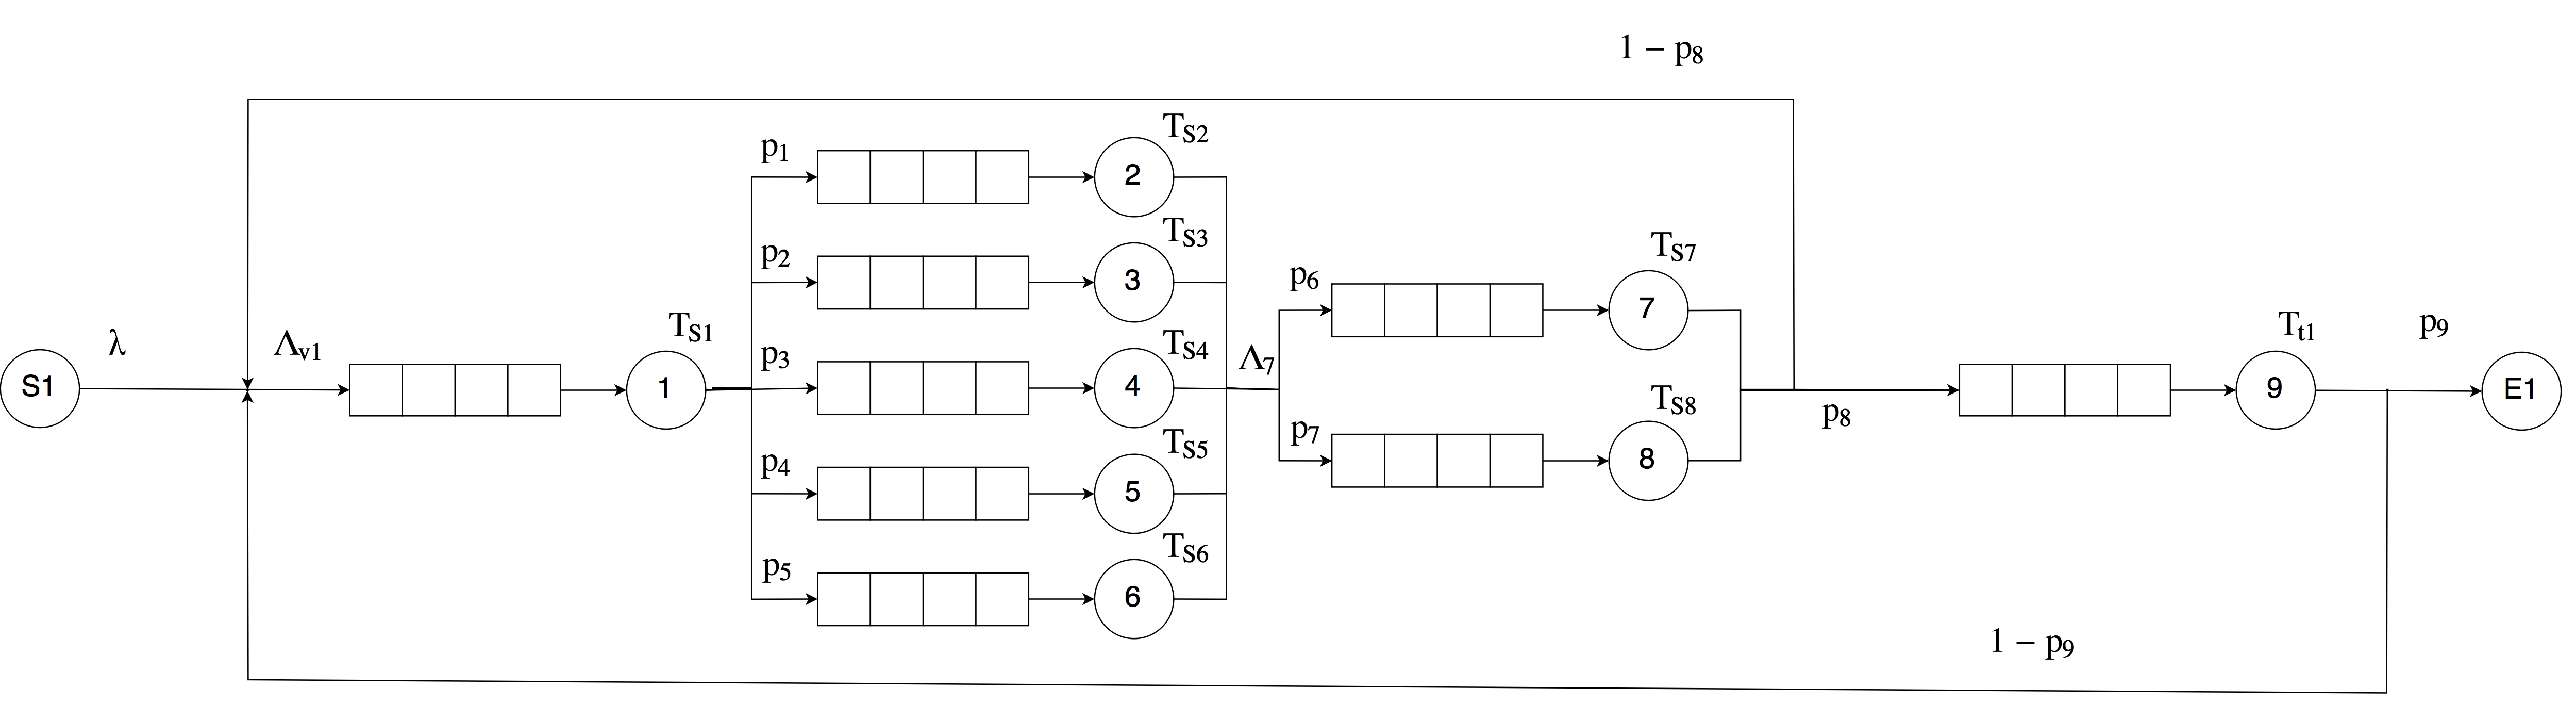
\includegraphics[width=1\linewidth]{menza_moje}
		\caption[Schéma navrženého modelut]{Schéma navrženého modelu}
		\label{fig:schema_menza}
	\end{figure}

\subsection{Naměřené hodnoty systému}

V rámci experimentu byly naměřeny střední hodnoty jako:

\begin{itemize}  
\item Počet strávníků, kteří přijdou za jednotku času - $\lambda$
\item Počet strávníků, kteří mohou projít přes turniket za jednotku času - $\mu_1$
\item Počet strávníků, kteří mohou projít přes pokladnu za jednotku času - $\mu_7$ a $\mu_8$
\item Počet strávníků, kteří mohou projít přes pokladnu za jednotku času - $\mu_7$ a $\mu_8$
\item Počet strávníků, kteří mohou projít přes stroj s tácy za jednotku času - $\mu_9$
\end{itemize}

Zbylé hodnoty, jako pravděpodobnosti výběru jídel ($p_1$ až $p_5$), doba jejich vydání ($\mu_1$ až  $\mu_5$), pravděpodobnost volby pokladny ($p_6$ až $p_7$), pravděpodobnost návratu na začátek po zaplacení jídla (1 - $p_8$) a pravděpodobnost návratu na začátek po odevzdání tácu  (1 - $p_9$), byly odhadnuty na základě předchozích zkušeností s tímto zařízením.
Hodnoty jsou shrnuty v tabulkách níže.

\begin{table} [ht!]
\centering
    \begin{tabular}{|l|l|}
    \hline
    Název & \\ \hline
    $\lambda_1$   & 12 \\ \hline
    \end{tabular}
\caption {Generátory požadavků}
\end{table}

\begin{table} [ht!]
\centering
    \begin{tabular}{|l|l|}
    \hline
   $\mu_1$     & 20 \\ \hline
    $\mu_2$  & 12 \\ \hline
    $\mu_3$     & 11 \\ \hline
    $\mu_4$     & 13 \\ \hline
    $\mu_5$     & 12 \\ \hline
    $\mu_6$      & 14 \\ \hline
    $\mu_7$      & 11 \\ \hline
    $\mu_8$      & 12 \\ \hline
    $\mu_9$      & 18 \\ \hline
    \end{tabular}
    \caption {Zpracovávající zařízení}
\end{table}

\begin{table} [ht!]
\centering
    \begin{tabular}{|l|l|}
    \hline
   $p_1$     & 0.15 \\ \hline
    $p_2$  & 0.25 \\ \hline
    $p_3$     & 0.18 \\ \hline
    $p_4$     & 0.19 \\ \hline
    $p_5$     & 0.23 \\ \hline
    $p_6$      & 0.55 \\ \hline
    $p_7$      & 0.45 \\ \hline
    $p_8$      & 0.96 \\ \hline
    $p_9$      & 0.96 \\ \hline
    \end{tabular}
    \caption {Pravděpodobnosti přechodů}
\end{table}



\section{Analytické řešení}

Nejprve je nutné vypočítat střední frekvenci přichodů požadavků pro všechny uzly. 
Výsledná střední frekvenci přichodů se vždy skládá z těch prodů, které do uzlu přitečou mínus ty proudy, které z uzlu odtečou.
Pro mnou navržený experiment jsou rovnice následující:



$$
\Lambda_1 = \lambda + (1 - P_{8}) \cdot (\Lambda_{7} + \Lambda_{8}) + (1 - P_{9}) \cdot \Lambda_{9}
$$
$$
\Lambda_{2} = P_1 \cdot \Lambda_{1} 
$$
$$
\Lambda_{3} = P_2 \cdot \Lambda_{1} 
$$
$$
\Lambda_{4} = P_3 \cdot \Lambda_{1} 
$$
$$
\Lambda_{5} = P_4 \cdot \Lambda_{1} 
$$
$$
\Lambda_{6} = P_5 \cdot \Lambda_{1} 
$$
$$
\Lambda_{7} = \Lambda_{2} + \Lambda_{3} + \Lambda_{4}  + \Lambda_{5} + \Lambda_{6} 
$$
$$
\Lambda_{8} = P_6 \cdot \Lambda_{7} 
$$
$$
\Lambda_{9} = P_7 \cdot \Lambda_{7} 
$$
$$
\Lambda_{10} = P_8 \cdot (\Lambda_{8} + \Lambda_{9}) 
$$

V rámci řešení této soustavy rovnic je klíčové vyjádřit $\Lambda_1$ v prvním řádku dosazením dalších neznámých z řádků ostatních. 
Vyjde nám tak rovnice, kde na jedné straně bude $\Lambda_1$ a na druhé vstupní proud $\lambda$, který známe ze zadání.
Pak už se jen dosazuje do dalších rovnic.

\begin{table} [ht!]
\centering
    \begin{tabular}{|l|l|}
    \hline
   $\Lambda_1$     & 13.02 \\ \hline
    $\Lambda_2$  & 1.95 \\ \hline
    $\Lambda_3$     & 3.20 \\ \hline
    $\Lambda_4$     & 2.35 \\ \hline
    $\Lambda_5$     & 2.47 \\ \hline
    $\Lambda_6$      & 3.02 \\ \hline
    $\Lambda_7$      & 7.16 \\ \hline
    $\Lambda_8$      & 5.85 \\ \hline
    $\Lambda_9$      & 12.5 \\ \hline
    \end{tabular}
    \caption {Analiticky vypočítané frekvence příchodů požadavků jednotlivých uzlů}
\end{table}

Jakmile máme určenou frekvenci příchodů požadavků všech uzlů a známe dobu, za jakou dobu umí jednotlivé uzly odbavit požadavek, můžeme spočítat jejich zatížení.
Díky tomu dokážeme určit, zda síť není zahlcená, tedy je ve stacionárním režimu a můžeme použít Littleovy vzorce pro další výpočty.

Zatížení uzlu se spočítá jako:

$$
	\rho = \frac{1}{m} \cdot \frac{\lambda}{\mu}
$$

tedy poměř střední hodnoty frekvence příchodu požadavků ku střední hodnotě frekvence doby obsluhy. $m$ reprezentuje počet obslužných kanálů. 
V našem případě je to 1.
Pokud jsou všechny hodnoty $ \rho $ menší než 1, je systém ve stacionárním režimu.

\begin{table} [ht!]
\centering
    \begin{tabular}{|l|l|}
    \hline
   $\rho_1$     & 0.65 \\ \hline
    $\rho_2$  & 0.16 \\ \hline
    $\rho_3$     & 0.29 \\ \hline
    $\rho_4$     & 0.18 \\ \hline
    $\rho_5$     & 0.20 \\ \hline
    $\rho_6$      & 0.21 \\ \hline
    $\rho_7$      & 0.65 \\ \hline
    $\rho_8$      & 0.48 \\ \hline
    $\rho_9$      & 0.69 \\ \hline
    \end{tabular}
    \caption {Zatížení jednotlivých uzlů}
\end{table}

Z výsledků tedy vyplývá, že můžeme pro výpočet dalších statistik použít Littleovy vzorce:

$$
L_q = \lambda \cdot T_q
$$
$$
L_w = \lambda \cdot T_w
$$
$$
T_w = L_w \cdot T_a
$$

$L_q$ je střední počet požadavků v celém systému hromadné obsluhy (SHO). Lze také vyjádřit jako:

$$
	L_q = L_w + L_s = L_w + m \cdot \frac{ \lambda }{ \mu }
$$

který nám říká, že v systému je to, co je ve frontě a v kanálech obsluhy.
Pokud se jedná o SHO klasifikace  M/M/1, je možné spočítat $L_q$ jako:

$$
L_q = \frac{\rho}{(1 - \rho)}
$$

S využitím tohoto vzorce si spočítáme střední počet požadavků pro všechny uzly.

\begin{table} [ht!]
\centering
    \begin{tabular}{|l|l|}
    \hline
   $Lq_1$     & 1.86 \\ \hline
    $Lq_2$  & 0.19 \\ \hline
    $Lq_3$     & 0.41 \\ \hline
    $Lq_4$     & 0.22 \\ \hline
    $Lq_5$     & 0.25 \\ \hline
    $Lq_6$      & 0.27 \\ \hline
    $Lq_7$      & 1.86 \\ \hline
    $Lq_8$      & 0.95 \\ \hline
    $Lq_9$      & 2.27 \\ \hline
    \hline
    $Lq$      & 8,29 \\ \hline
    \end{tabular}
    \caption {Střední počet požadavků v uzlech}
\end{table}

Pokud sečteme dílčí výsledky, vyjde nám střední počet požadavků pro celý systém tedy $L_q = 8,29$.

$T_q$, neboli střední doba odezvy systému SHO lze vyjádřit jako:
$$
T_q = T_w + T_s = T_w + \frac{1}{\mu}
$$

V našem případě lze využít Littleova vzorce a vypočítat střední dobu odezvy jako střední počet požadavků v systému děleno střední frekvencí příchodu požadavků, tedy $T_q = 0.69$




\section{Řešení simulačním programem}%%%%%%%%%%%%%%%%%%%%%%%%%%%%%%%%%%%%%%%%%%%%%%%%%%%%%%%%%%%%%%%%%%%%%%%%%%%%%%%%%%%%%%%%%%%%%%%%%%%%%%%%%%%%%%%%%%%%%%%%%%%%%%%%%%%%%%%%%%

\subsection{Použité nástroje a jazyky}
Pro řešení jsem se rozhodl využít simulační knihovnu J-Sim, která je napsána v jazyce Java a je možné tak využít objektově orientované programování.
Alternativou bylo použít knihvnu C-Sim, který je psán pro ANSI C.

\subsection{Generování náhodných čísel}

Jedním z požadavků semestrální práce bylo umožnit generovat nově příchozí požadavky s Gaussovským rozdělením.
Pro vygenerování pseudonáhodných čísel s Gaussovým rozdělením byla navržena metoda Box-Mullerovi transformace \cite{box1958note}.
Tato metoda je navržena tak, že během jednoho běhu vrací dvě pseudonáhodná čísla (\( Z_0 \) a (\( Z_1 \)). 
Vstupem metody jsou dvě náhodná čísla -- \( U_1 \) a \( U_2 \) -- s uniformním rozdělením uvnitř intervalu \( (0,1) \).
Samotný výpočet výsledných pseudonáhodných čísel je pak následující:


\begin{equation} 
Z_0 = R\cos{(\theta)} \sqrt{-2\ln{U_1}}\cos{(2\pi U_2)}
\end{equation}

\begin{equation} 
Z_1 = R\sin{(\theta)} \sqrt{-2\ln{U_1}}\sin{(2\pi U_2)}
\end{equation}


\subsubsection{Výpočet statistik za běhu}

Střední hodnotu Gaussova rozdělení je možné vypočítat jako:

\begin{equation} 
\overline{x} = \frac{1}{n}(\sum_{i=1}^{n}x_i)
\end{equation}

a směrodatnou odchylku jako:
\begin{equation} 
s = \sqrt{\frac{\sum_{i=1}^{N}(x_i - \bar{x})^2}{N - 1}}
\end{equation}

Pro realizaci těchto výpočtů je ale nutné si všechna vygenerovaná čísla ukládat.
Pro přepočet střední hodnoty po vygenerování nového pseudonáhodného čísla je v tomto případě možno použít:

\begin{equation} 
\bar{x}_n = \frac{n\bar{x}_{n-1} + x_{new}}{n+1}
\end{equation}

kde \( n \) je počet vygenerovaných čísel, \( \bar{x}_{n-1} \) je stará střední hodnota a \( \bar{x}_{new} \)  je nově vygenerované číslo.

Pro přepočet rozptylu je to pak:
\begin{equation} 
\sigma^{2}_{new} = \frac{n(\sigma^{2}_{old}+ \bar{x}^2) + x^{2}_{new}}{n+1} - \bar{x}^{2}_{new} 
\end{equation}

kde \( n \) je počet vygenerovaných čísel, \( \sigma^{2}_{old} \) je hodnota staré odychlky,  \( x_{new} \) je nově vygenerované číslo a \( \bar{x}^{2}_{new}  \) je střední hodnota získaná z předchozí rovnice.


Pro vygenerování pseudonáhodných čísel s Gaussovým rozdělením byla navržena metoda Box-Mullerovi transformace \cite{box1958note}.
Tato metoda je navržena tak, že během jednoho běhu vrací dvě pseudonáhodná čísla (\( Z_0 \) a (\( Z_1 \)). 
Vstupem metody jsou dvě náhodná čísla -- \( U_1 \) a \( U_2 \) -- s uniformním rozdělením uvnitř intervalu \( (0,1) \).
Samotný výpočet výsledných pseudonáhodných čísel je pak následující:


\begin{equation} 
Z_0 = R\cos{(\theta)} \sqrt{-2\ln{U_1}}\cos{(2\pi U_2)}
\end{equation}

\begin{equation} 
Z_1 = R\sin{(\theta)} \sqrt{-2\ln{U_1}}\sin{(2\pi U_2)}
\end{equation}

Zde je ukázka histogramu z algoritmu mnou implementovaným. Vstupním parametrem byla střední hodnota 1000 a odchylka 10 a vygeneroval se celkem jeden milion čísel.\\\\
\texttt
{
E\_teorie=1000.0\\
D\_teorie=100.0\\
E\_vypocet=1000.0369173235879\\
D\_vypocet=98.70743444378536\\
733,33:*\\
766,67:**\\
800,00:*****\\
833,33:*********\\
866,67:***************\\
900,00:*********************\\
933,33:**************************\\
966,67:*****************************\\
1000,00:*****************************\\
1033,33:**************************\\
1066,67:*********************\\
1100,00:***************\\
1133,33:**********\\
1166,67:*****\\
1200,00:**\\
1233,33:*\\
}

Z výsledků je vidět, že je teoretická hodnota blízská hodnotě ze simulace.


\subsection{Implementace}
Místem spuštění celého programu je třída Main. 
Ta přečtě vstup od uživatele a spustí podle toho simulaci s patřičnými parametry.
Dále je implementace rozdělená do několika balíků

\subsubsection{Request}
V tomto balíku jsou třídy, reprezentující požadavek, který běží systémem (\texttt{Request}). 
\subsection{Výsledky}

\section{Porovnání výsledků}

\section{Uživatelská příručka}

\section{Závěr} %%%%%%%%%%%%%%%%%%%%%%%%%%%%%%%%%%%%%%%%%%%%%%%%%%%%%%%%%%%%%%%%%%%%%%%%%%%%%%%%%%%%%%%%%%%%%%%%%%%%%%%%%%%%%%%%%%%%%%%%%%%%%%%%%%%%%%%%%%
V rámci úkoly byly vypočítány střední frekvence jednotlivých uzlů, jejich zatížení, střední délka fronty a střední doba obsluhy. Následně bylo vypočítáno, kolik procent časového intervalu sledování bude druhá fronta prázdná. Společně s úkolem je navíc odevzdán soubor s daty pro program QNAlyzer pro případnou kontrolu.
\end{document}